
\chapter{Menu surfaces}
\minitoc 


In most cases, these function only apply on selected surfaces, so, as a prerequisite, you almost always need to select surfaces in order to use what is described below.



\section{Structure modification}
\subsection{Smooth each selected surface}
\noindent
\begin{minipage}{0.5\textwidth}
This option uses vtkSmoothPolyDataFilter.You may smooth an input
selected surface using this option (see Fig. \ref{smooth}). A number of iteration and a
relaxation factor are required.\\
See vtkSmoothPolyDataFilter documentation for further information regarding this option.
\end{minipage}    
\begin{minipage}{0.5\textwidth}\centering
  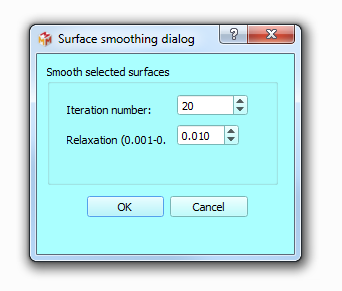
\includegraphics[scale=0.5]{images/09/structure/surface_smoothing_dialog.png}
 \captionof{figure}{Surface smoothing window}
 \end{minipage} 
\noindent

\begin{figure}
  \centering
  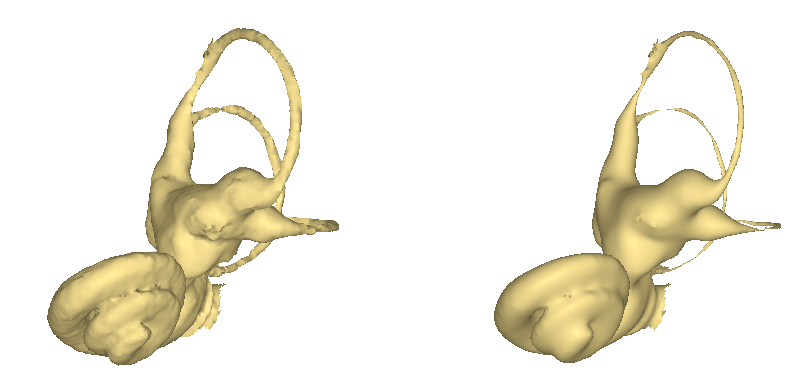
\includegraphics[scale=0.5]{images/Edit_selected_objects/05_smooth.png} 
	\caption{Left: example of original input surface. Right: resulting output surface after 50 iterations using a relaxation factor of 0.1.}
\label{smooth}
 
\end{figure}

\subsection{Invert}

A given surface's triangles can be
inverted in order to show inner structures (see Fig. \ref{inversion}).\\

Note that the original surface
is directly affected; this option
does not involve the use of a
filter (no output additional
surface is created).


\begin{figure}
  \centering
  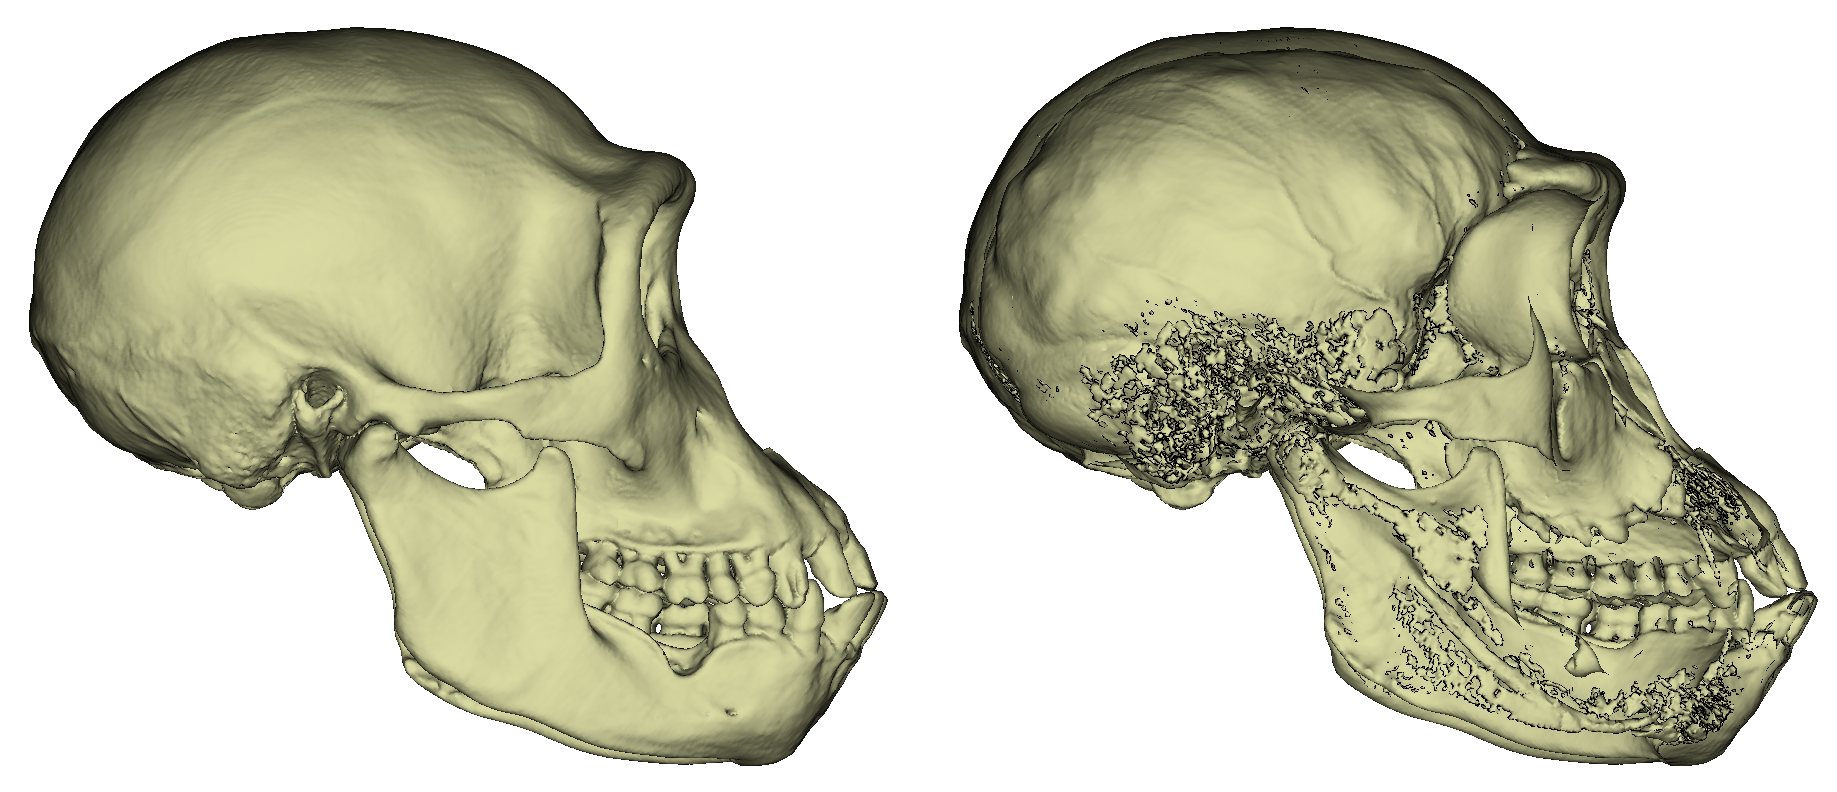
\includegraphics[scale=0.4]{images/Edit_selected_objects/01_invert.png} 
	\caption{Example of surface triangle inversion. Left: original surface.
Right: the same surface inverted, revealing inner structures such
as the endocranial cavity. Gouraud shading rendering + backface
culling option was used.}
\label{inversion}
 
\end{figure}






\subsection{Mirror}

This option uses vtkReflectionFilter,which produces a mirror image of the original selected input mesh (see Fig. \ref{mirror}).\\

\begin{figure}
  \centering
  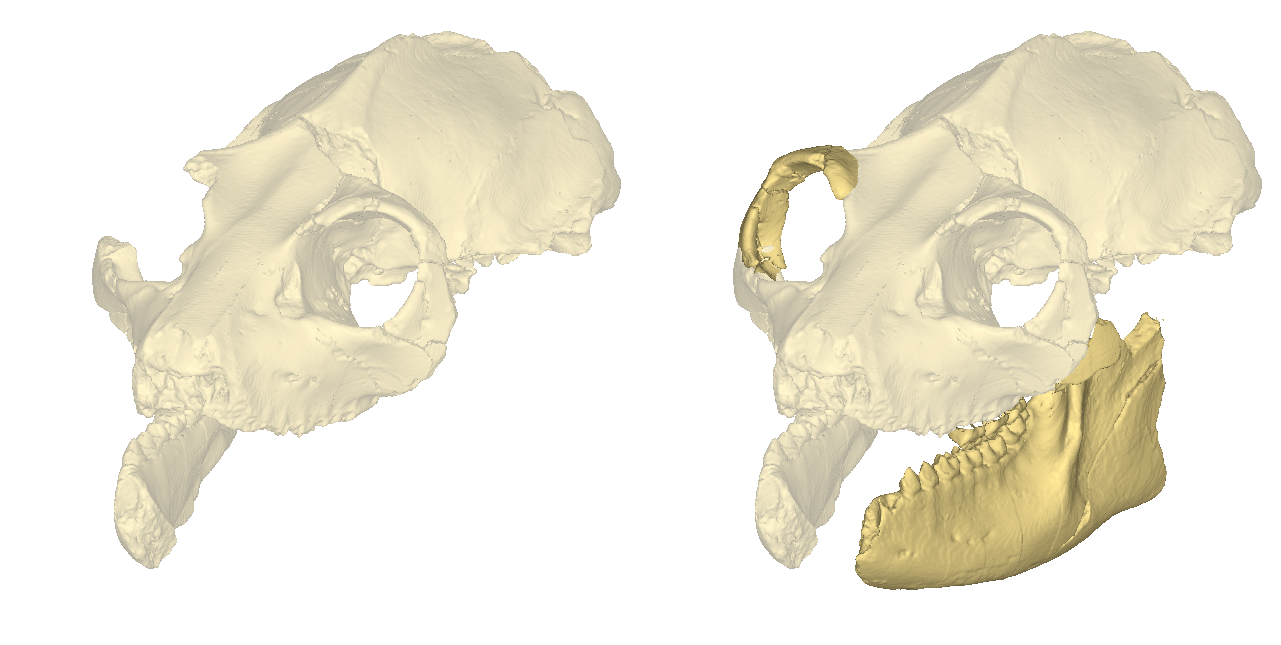
\includegraphics[scale=0.35]{images/Edit_selected_objects/02_Mirror.png} 
	\caption{Example of fossil restoration implicating the production of mirror images of missing parts.}
 \label{mirror}
\end{figure}

\subsection{Connectivity : separate all non connected regions}
\noindent
\begin{minipage}{0.5\textwidth}
This option uses vtkPolyDataConnectivityFilter. This filter produces a new surface for each non-connected region of the selected input surface. 3D meshes of biological objects sometimes contain a multitude of small and biologically irrelevant independent regions. This ``noise" may have multiple origins: low quality of original 3D data, state of preservation of the specimen, threshold used to be able to visualize all relevant structures, etc... In order to extract relevant independent regions, only regions reaching a minimal size (minimal number of triangles) are transformed into new surfaces (see Fig. \ref{decompose34}). This process may take some time to be completed. All produced surfaces corresponding to independent regions can be manipulated independently (see Fig. \ref{decompose5}).\end{minipage}    
\begin{minipage}{0.5\textwidth}\centering
  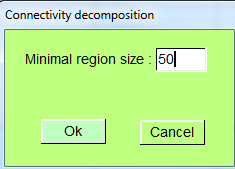
\includegraphics[scale=0.5]{images/Edit_selected_objects/03_Decompose.png}
 \captionof{figure}{Connectivity decomposition window}
 \end{minipage} 
\noindent


\begin{figure}
  \centering
  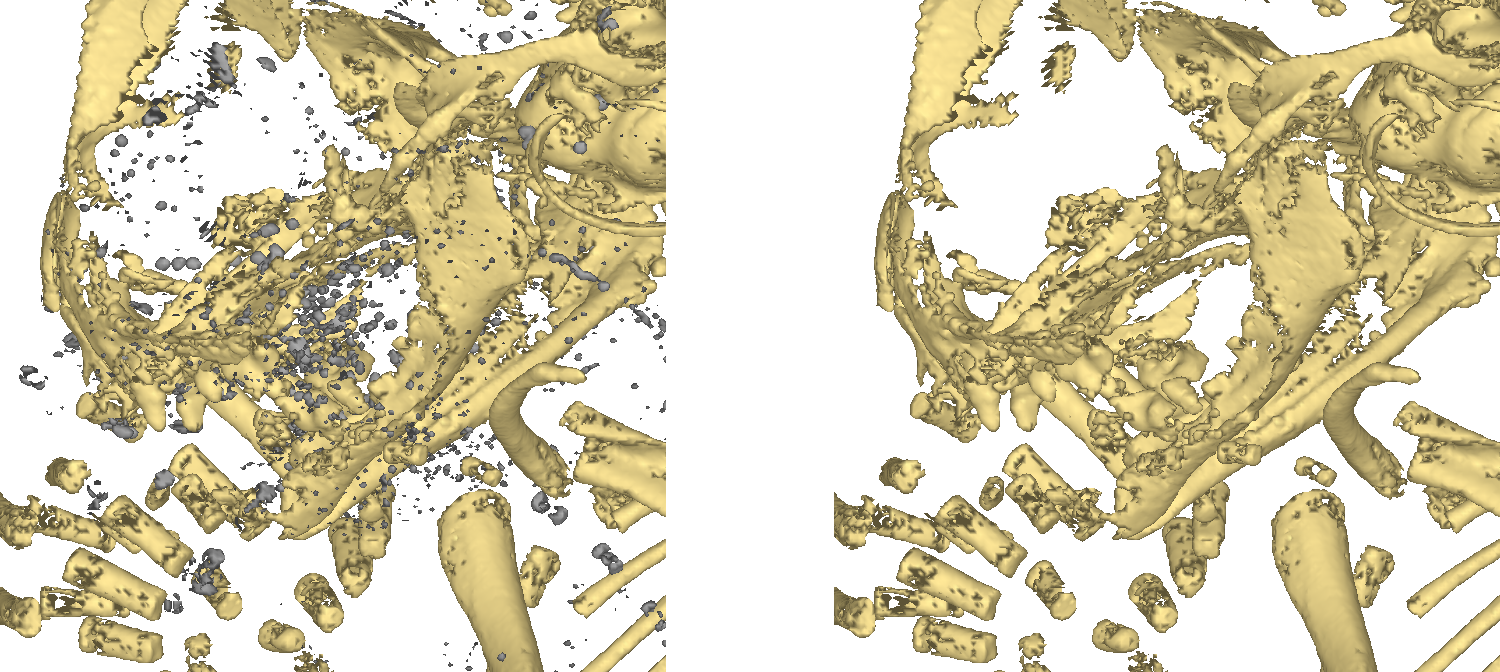
\includegraphics[scale=0.3]{images/Edit_selected_objects/03_Decompose_34.png} 
	\caption{Left: Original surface containing a large number of independent regions of size greater than 350 triangles (in grey). Right : Filtered surfaces. All meshes produced using this filter have more than 350 triangles.}
\label{decompose34}
 
\end{figure}

\begin{figure}
  \centering
  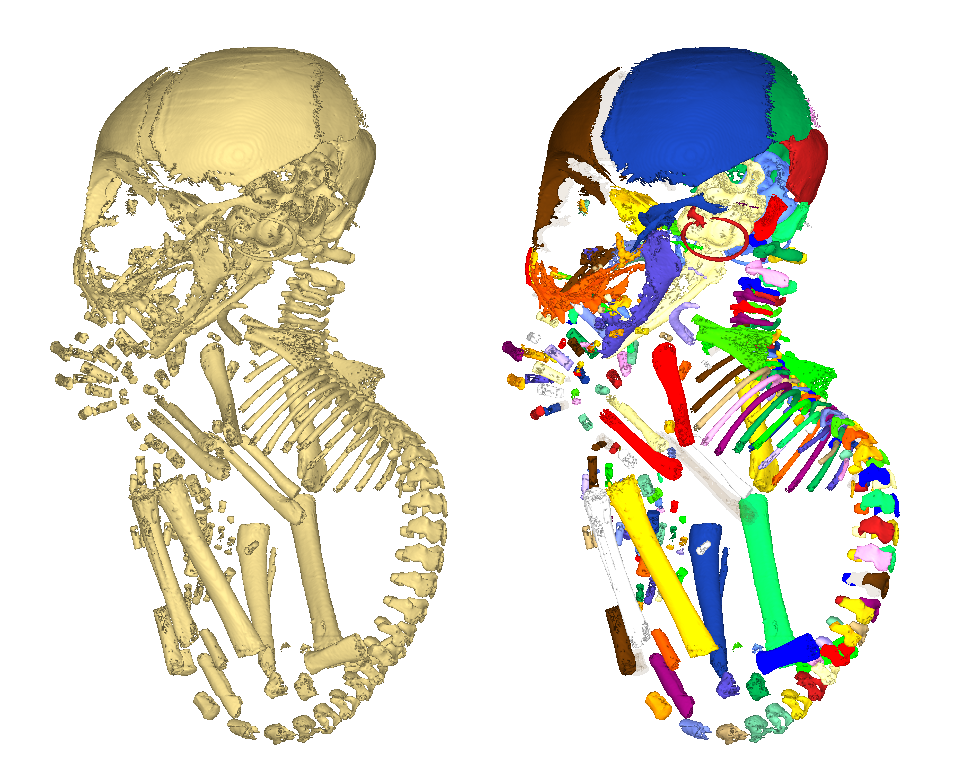
\includegraphics[scale=0.4]{images/Edit_selected_objects/03_Decompose5.png} 
	\caption{Left: original surface (one single mesh). Right: the resulting 298 filter output surfaces (each drawn using a different color) can be manipulated independently.}
\label{decompose5}
 
\end{figure}





\subsection{Connectivity: keep largest region}
This option uses vtkPolyDataConnectivityFilter.This filter produces a new surface for the largest independent region of the selected input surface (see Fig. \ref{largest_region}).

\begin{figure}
  \centering
  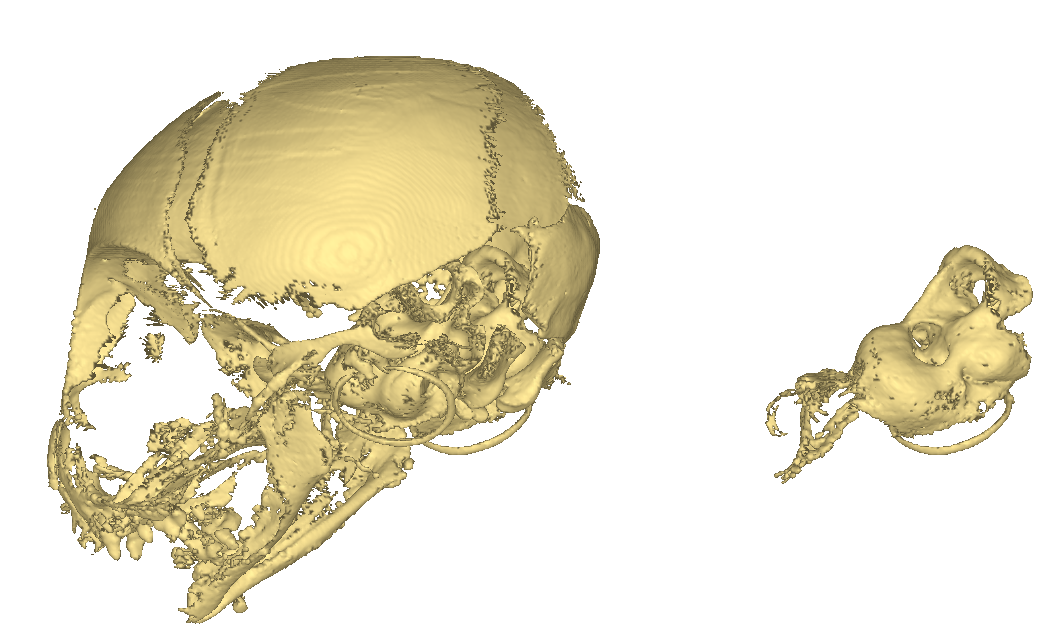
\includegraphics[scale=0.4]{images/Edit_selected_objects/03_Decompose6.png} 
	\caption{Left: original surface. Right: the resulting largest region in terms of triangle number.}
\label{largest_region}
 
\end{figure}









\subsection{TPS deformation}
\noindent
\begin{minipage}{0.5\textwidth}
This option uses vtkThinPlateSplineTransform filter.
Requirements : to use TPS deformation, a selected surface,
a series of ``n" normal landmarks and a series of ``n"
target landmarks (n>3) are needed. ``Normal" landmarks
are usually placed on the original selected input surface,
whereas ``target" landmarks are placed at a location in 3D
space which will drive the TPS deformation (see Fig. \ref{tps}). See vtkThinPlateSplineTransform documentation for further information regarding TPS deformation.

\end{minipage}    
\begin{minipage}{0.5\textwidth}\centering
  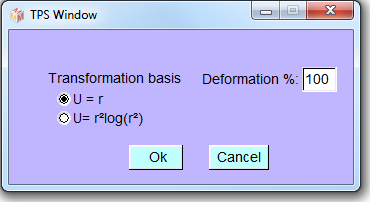
\includegraphics[scale=0.5]{images/Edit_selected_objects/06_tps.png}
 \captionof{figure}{TPS window}
 \end{minipage} 
\noindent

\begin{figure}
  \centering
  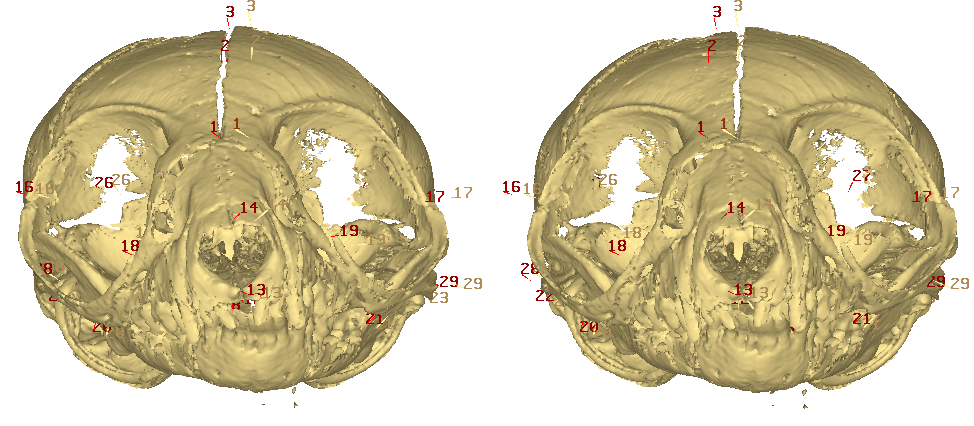
\includegraphics[scale=0.5]{images/Edit_selected_objects/06_tps_input_output.png} 
	\caption{Left: original distorted input surface. 31 ``normal"
landmarks were placed on the surface and 31
``target" landmarks were placed in order to
restore bilateral symmetry. Right: resulting output (deformation : 100\%). Note
that the 31 ``target" landmarks are located on the output surface.
}
\label{tps}
 
\end{figure}





\subsection{Decimate}
\noindent
\begin{minipage}{0.5\textwidth}


This option uses vtkDecimatePro and vtkQuadricDecimation filters. Requirements : to use mesh decimation, a selected
surface is required (see for instance Fig. \ref{decimate}). See vtkDecimatePro and vtkQuadricDecimation documentations for further information regarding
mesh decimation.

\end{minipage}    
\begin{minipage}{0.5\textwidth}\centering
  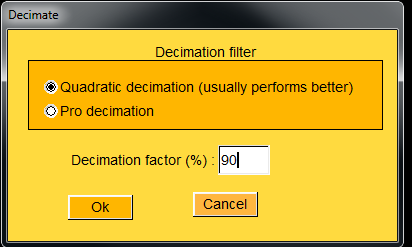
\includegraphics[scale=0.5]{images/Edit_selected_objects/07_decimate.png}
 \captionof{figure}{Decimate window}
 \end{minipage} 
\noindent

\begin{figure}
  \centering
  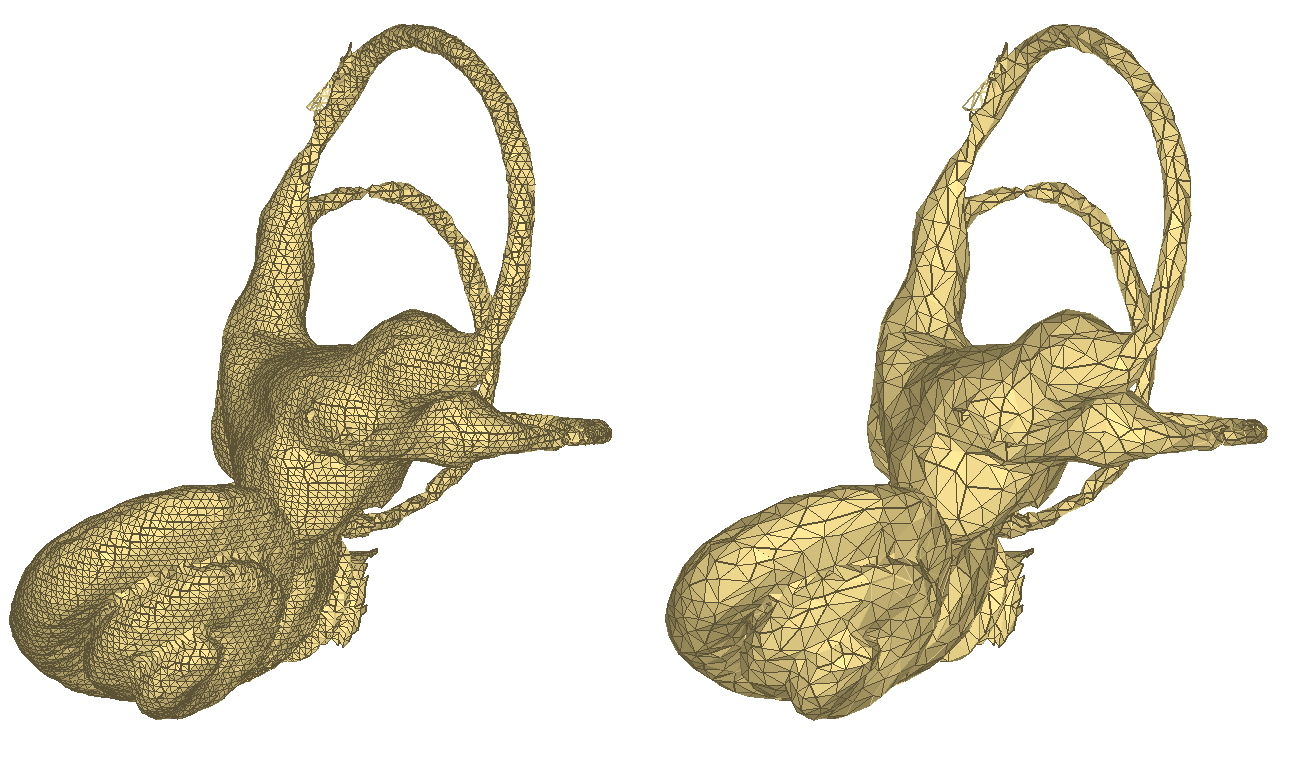
\includegraphics[scale=0.25]{images/Edit_selected_objects/07_decimate_input_output.png} 
	\caption{Mesh decimation. Left: original input surface. Number of triangles: 27679. Right: resulting output (vtkQuadricDecimation filter,
decimation factor: 80\%). Number of triangles:5535.
}
\label{decimate}
 
\end{figure}




\subsection{Densify}

\noindent
\begin{minipage}{0.5\textwidth}

This option uses vtkDensifyPolyData filter.
Requirements : to use mesh densification, a selected
surface is required (see for instance Fig. \ref{densify}).
Note that mesh decimation can become extremely slow
when using number of subdivisions larger than 1.
See vtkDensifyPolyData documentation for further information regarding mesh densification.

\end{minipage}    
\begin{minipage}{0.5\textwidth}\centering
  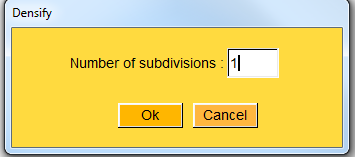
\includegraphics[scale=0.5]{images/Edit_selected_objects/08_densify.png}
 \captionof{figure}{Densify window}
 \end{minipage} 
\noindent

\begin{figure}
  \centering
  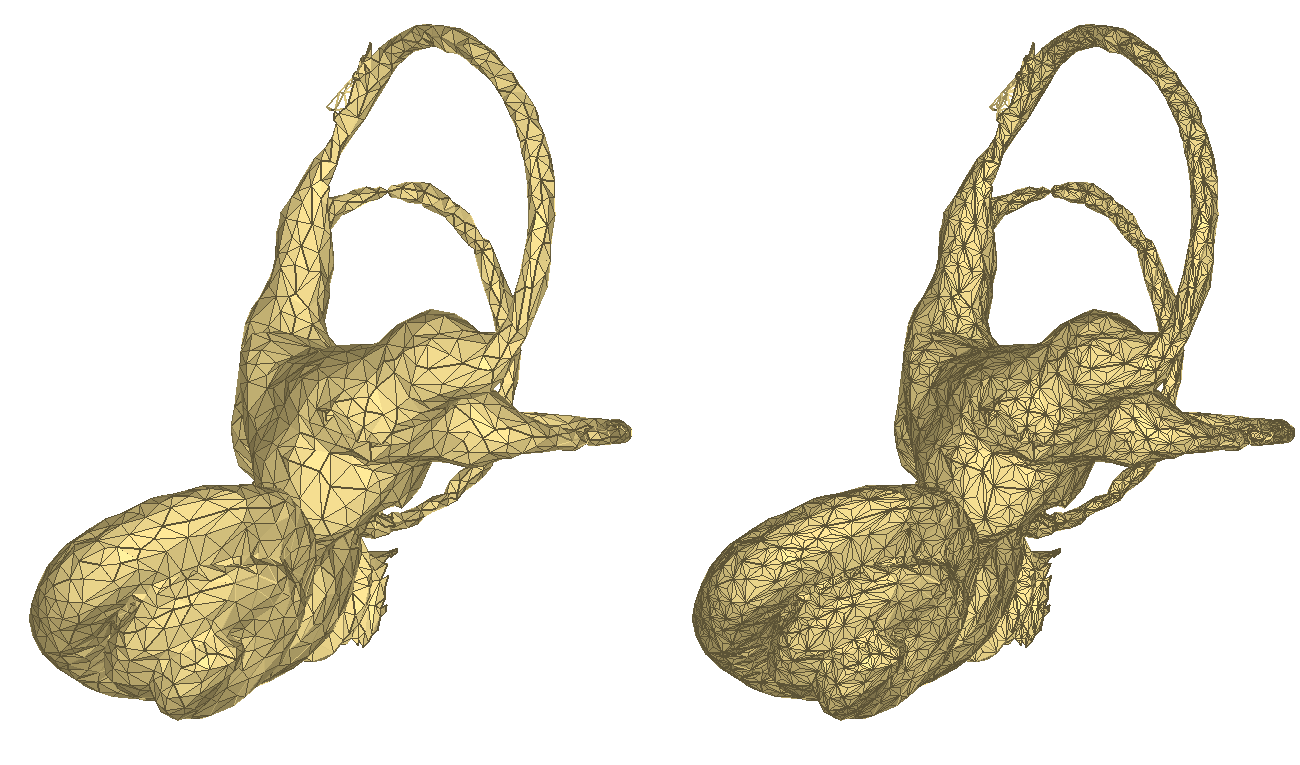
\includegraphics[scale=0.25]{images/Edit_selected_objects/08_densify_input_output.png} 
	\caption{Mesh densification. Left: original input surface. Number of triangles: 5535. Right: resulting output (number of subdivisions: 1). Number of triangles: 16605.
}
\label{densify}
 
\end{figure}




\subsection{Fill holes}

\noindent
\begin{minipage}{0.5\textwidth}

This option uses vtkFillHolesFilter.
Requirements : to use mesh hole filling, a selected surface is
required (see for instance Fig. \ref{fill_holes}). See vtkFillHolesFilter documentation for further
information regarding hole filling.


\end{minipage}    
\begin{minipage}{0.5\textwidth}\centering
  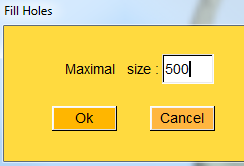
\includegraphics[scale=0.5]{images/Edit_selected_objects/09_fill_holes.png}
 \captionof{figure}{Fill holes window}
 \end{minipage} 
\noindent

\begin{figure}
  \centering
  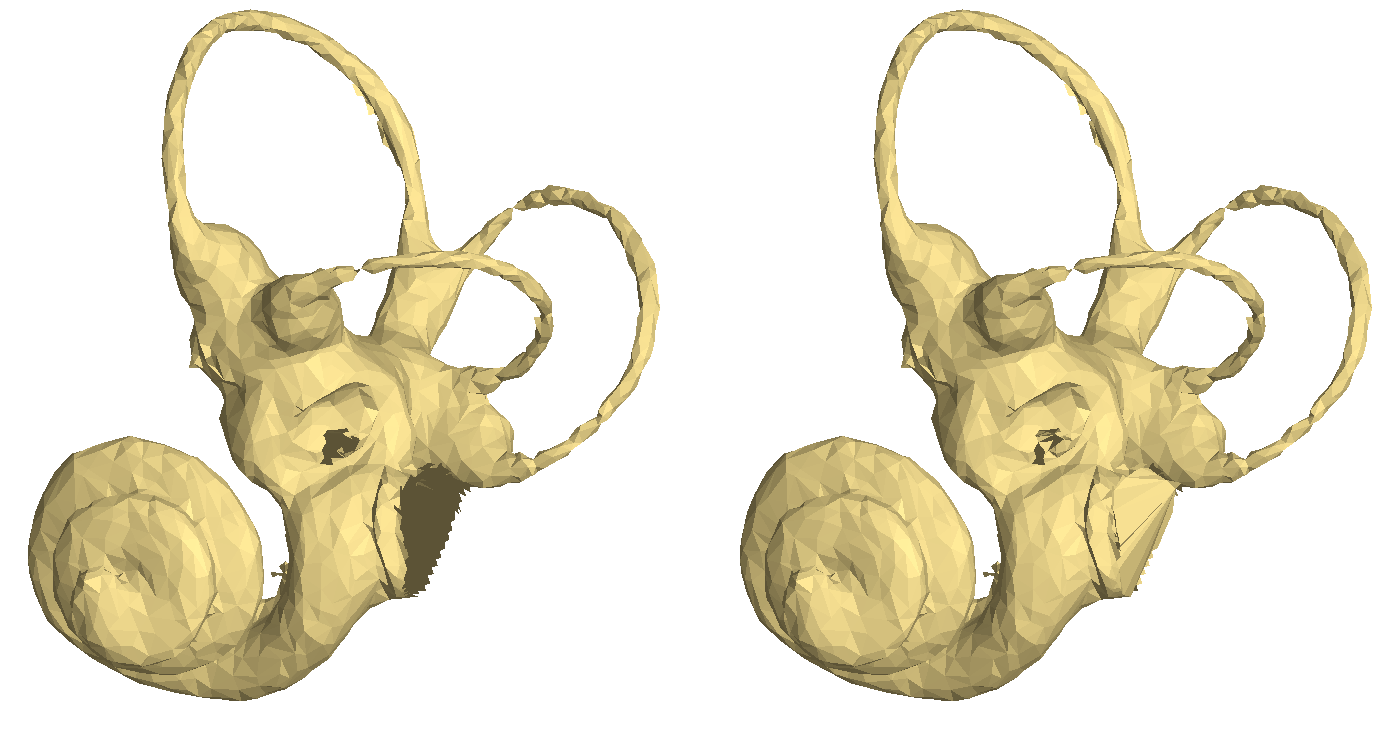
\includegraphics[scale=0.25]{images/Edit_selected_objects/09_fill_holes_input_output.png} 
	\caption{Filling holes. Left: original input surface. Number of triangles: 5535. Right: resulting output (maximal size: 1). Number of triangles: 5689.}
\label{fill_holes}
 
\end{figure}


\subsection{Registration ICP}
This option was implemented by Cécile Peladan, and deserves a chapter of its own and a tutorial, which will be written in a near future. 

\section{Rendering modifications.}
\subsection{Set alpha value}
\noindent
\begin{minipage}{0.5\textwidth}

A selected surface is needed.\\
Please chose a value between 0 and 100. 100 stands for ``opaque
rendering". 0 stands for ``invisible surface".\\


\end{minipage}    
\begin{minipage}{0.5\textwidth}\centering
  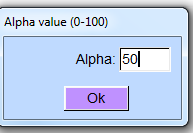
\includegraphics[scale=0.5]{images/Edit_selected_objects/10_transparency.png}
 \captionof{figure}{Alpha value setting window}
 \end{minipage} 
\noindent




As stated earlier, vertex display order has consequences on 3D rendering when working with
transparency. 3D objects are displayed one after the other following an object list. The way object are ordered inside this list thus affects transparency rendering, especially when some objects such as inner structures are positioned inside others. Object display order of selected objects can be changed using the two following controls. Pressing ``
\includegraphics[scale=0.7]{images/pixmap/s_dessous_17.png}" will place all selected objects one step earlier in the object display list. Pressing ``
\includegraphics[scale=0.7]{images/pixmap/s_dessus_17.png}" will place all selected objects one step further in the object display
list (see for instance Fig. \ref{transparency}). \\

See also ``Sort vertices from back to front (beware: slow rendering)"  (section \ref{sort_back_front}) and ``Sort vertices from front to back (beware: slow rendering)" (section \ref{sort_front_back}) for further information.\\

\begin{figure}
  \centering
  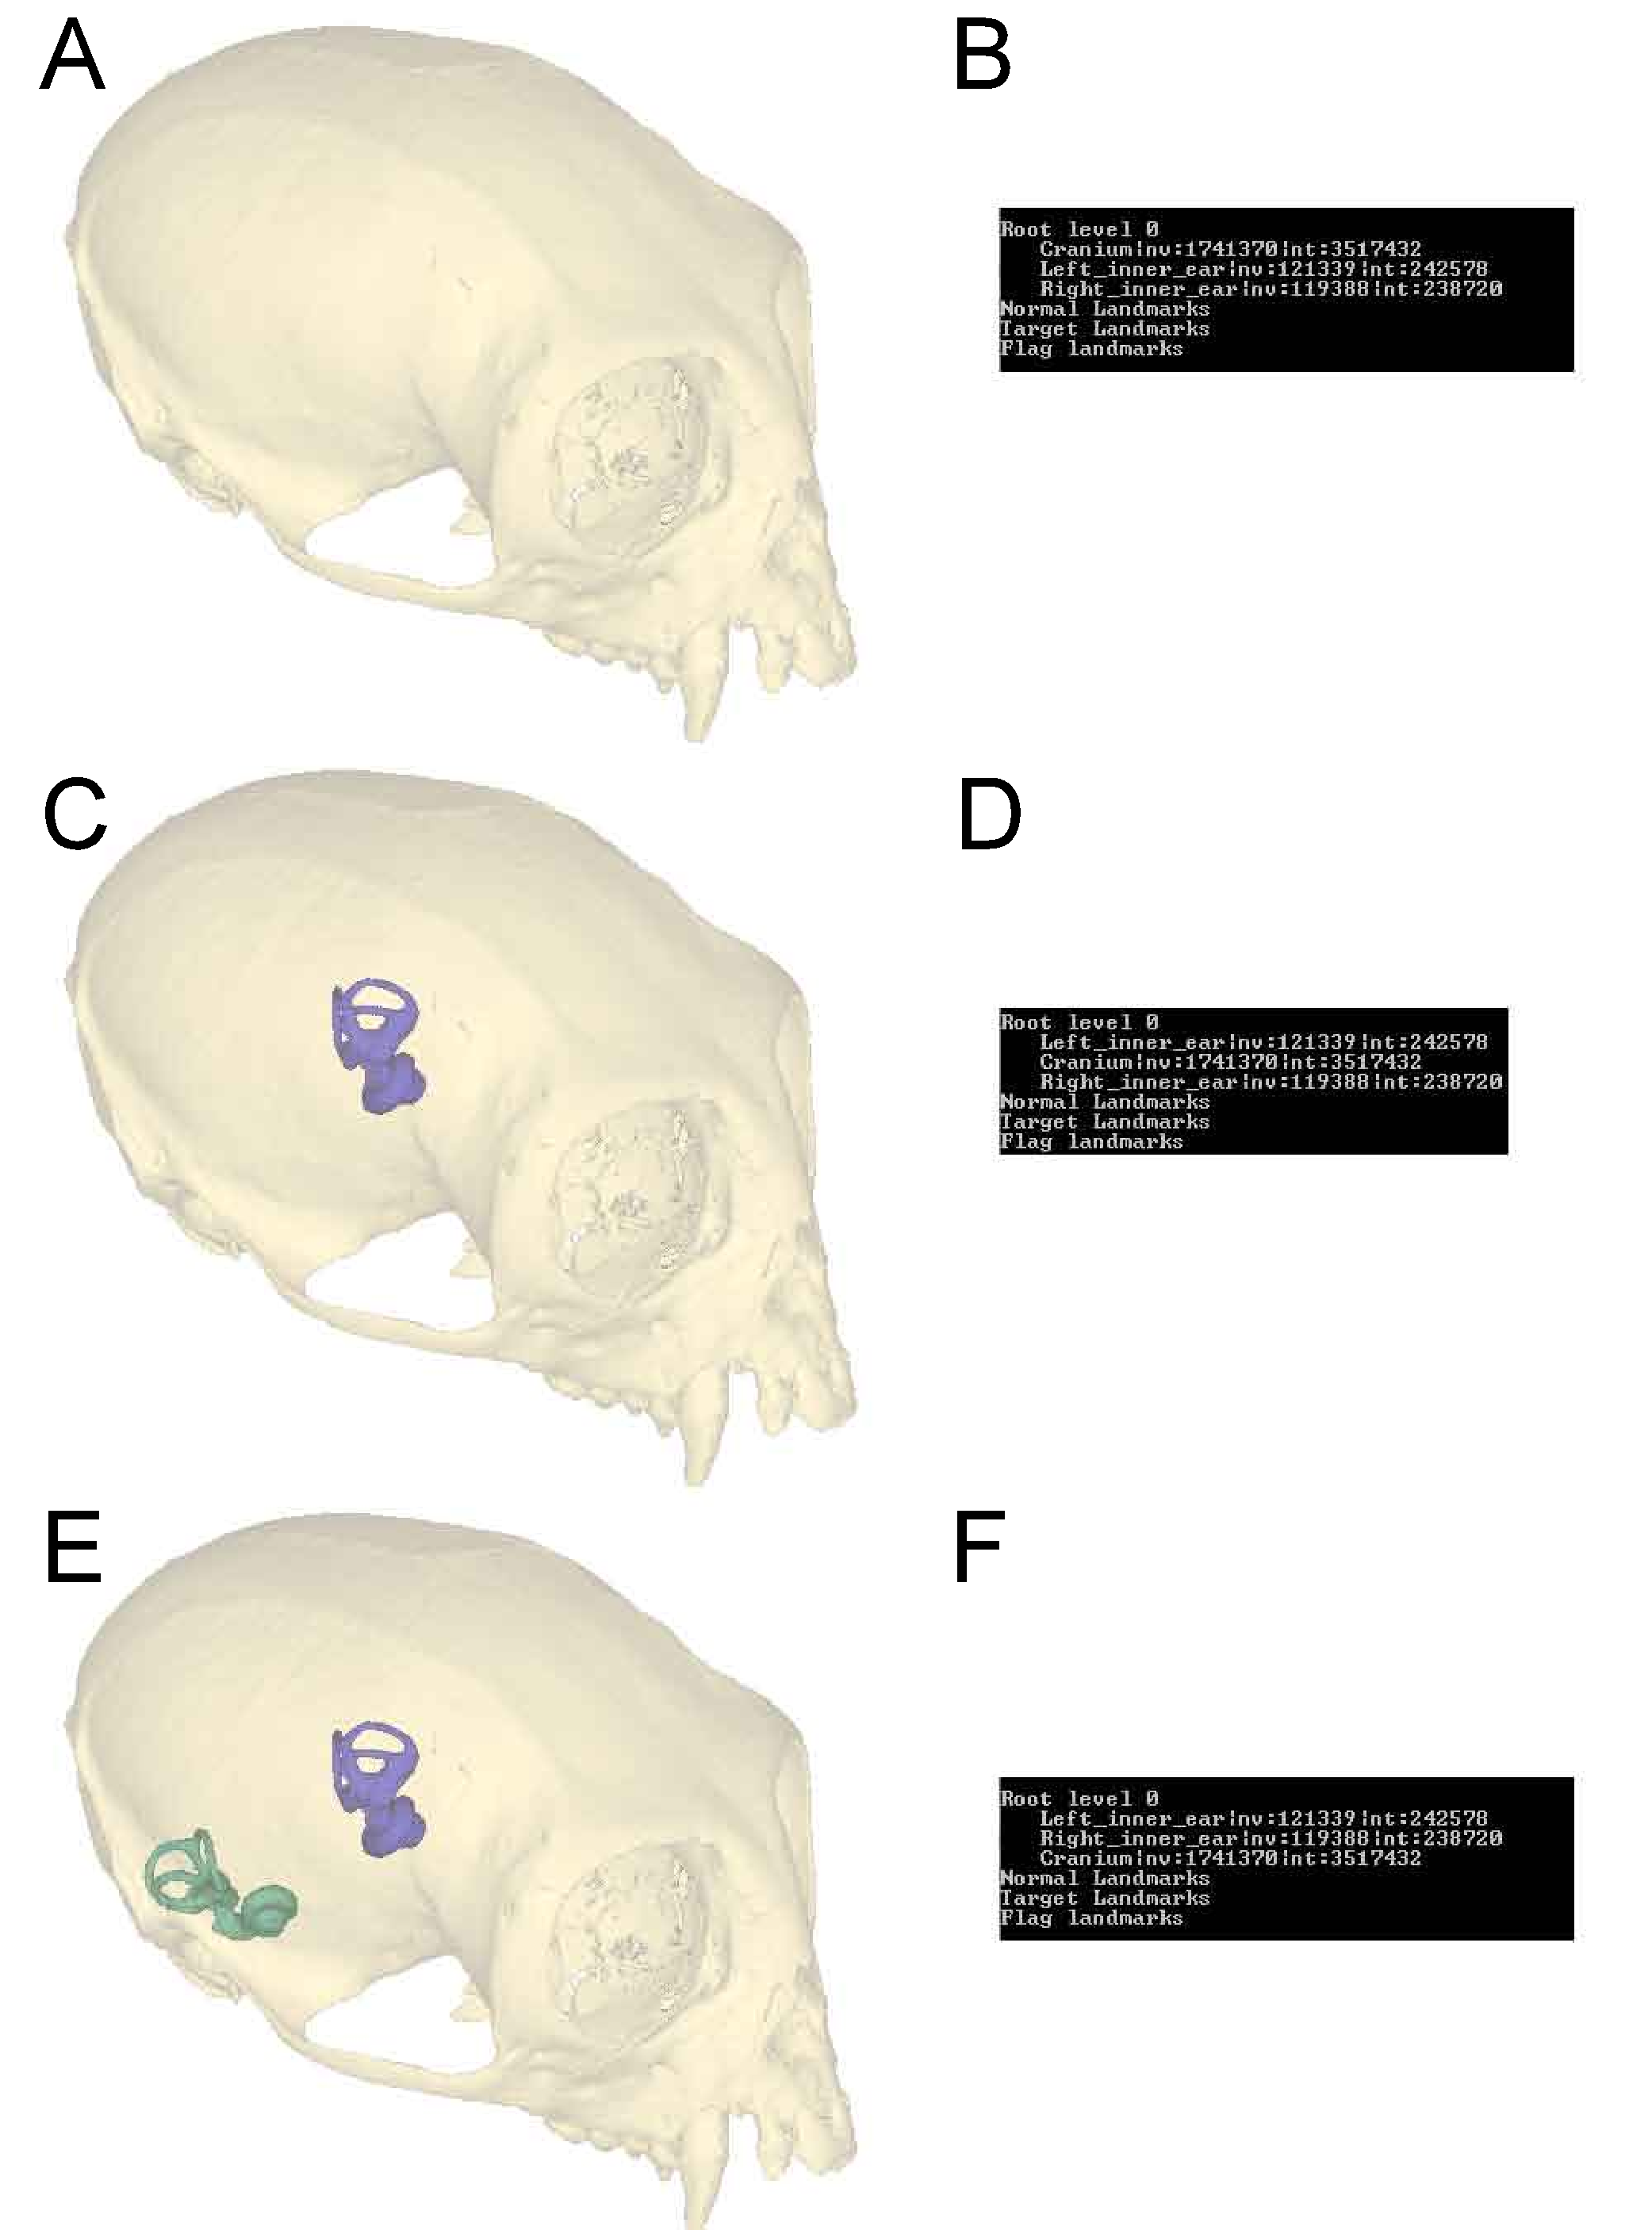
\includegraphics[scale=0.4]{images/Transparency/Transparency.pdf} 
	\caption{Transparency rendering. A. 3 objects (cranium, left\_inner\_ear and right\_
inner\_ear) are opened in this order, and the object ``cranium" is rendered with an alpha value of 40.
The inner ears remain invisible, because ``cranium" is displayed before the two inner ears are. B: corresponding display object order (Show $\rightarrow$Display
object order). C: the object ``Cranium" was selected and put downward in the object display list. Now the left inner ear is visible, as it is displayed before the cranium is. D: corresponding display object order. E: the object ``Cranium" was selected again, and put downward in the object display list. Now the two inner ears are
visible, because they are both rendered before the cranium is. F: corresponding display object order.}
\label{transparency}
 
\end{figure}




\subsection{Change object color}
Object color can be changed using this option. A set of 13 predefined colors is available via this menu. Alternatively, you can edit object color manually using the ``Object color" control of the ``General options" window (click on menu ``Show $\rightarrow$General options$\rightarrow$").

\subsection{Edit first selected object and aspect matrices}\label{edit_mat_section}

\noindent
\begin{minipage}{0.6\textwidth}

A selected surface is required . This opens the following window,
in which the aspect and position matrices can be edited.
Options :\\
- Ok : set aspect and position matrices to first selected object.\\
- Init : set aspect and position matrices to identity.\\
- Refresh : change matrices to those of first selected object.\\
- Ok for all selected objects: set aspect and position matrices to
all selected objects.\\
You can also access faster the ``Object Matrix" window by clicking
on ``
\includegraphics[scale=0.7]{images/pixmap/mat.png}"(edit first selected object position and aspect matrices).

\end{minipage}    
\begin{minipage}{0.4\textwidth}\centering
  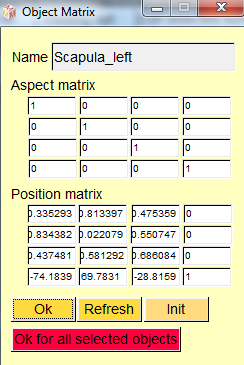
\includegraphics[scale=0.5]{images/File/Position2.png}
 \captionof{figure}{Object matrix window}
 \end{minipage} 
\noindent



\section{Grouping actions.}
One or several meshes can be placed into one logical object using this option. This option is useful in the following two cases.\\
- It allows an easy way to select/unselect together several objects (sometimes you do not want
to select/unselect manually multiple meshes one by one).\\
- As a logical object's aspect object and position matrices can be edited, placing 1 or several
meshes into one logical object provides a convenient means to achieve deformation into
a particular direction in 3D space (for instance to achieve mesh decompression in one
direction, see for instance Fig. \ref{grouping}).\\
Logical objects can be also put into another logical object. Note that meshes contained into selected logical objects cannot be saved until they are ungrouped.

\subsection{Group}
Select one or several meshes. Click on ``Edit selected surfaces$\rightarrow$Grouping actions$\rightarrow$Group". As a result, the selected meshes are drawn in brown color.
\subsection{Ungroup}
Select one logical object. Click on ``Edit selected surfaces$\rightarrow$Grouping actions$\rightarrow$Ungroup". If the logical object aspect and position matrices are different from the identity matrices, the position and aspect matrices of the contained objects are edited in order to take into account position and aspect transformations that were applied to that logical object. Then the objects contained into the selected logical object are ungrouped, and the selected logical object is deleted.\\


\begin{figure}
  \centering
  \includegraphics[scale=0.25]{images/Edit_selected_objects/11_group.pdf} 
	\caption{
Grouping objects. A1: 7 objects are opened. Original matrices of ``bx\_md" object are shown (right mandible, selected). A2: corresponding display object order (Show $\rightarrow$Display object order). B1: The 7 object are grouped. The group is drawn in brown. B2: corresponding display object order. C1: the position of the group is changed, as well as its aspect matrix. Note that the enclosed meshes cannot be saved in that state. C2: corresponding display object order. D1: objects are ungrouped. Modified matrices of ``bx\_md" object are shown (right mandible is selected). Now, the 7 meshes can be saved. D2: corresponding display object order (Show $\rightarrow$Display object order).}
\label{grouping}
 
\end{figure}


\section{Object list order.}
As explained earlier, the following options are useful when working with transparent objects. Normal and Target landmark ordering can also be edited using these options.
\\As stated above, access to object display order can be reached via the menu ``Show$\rightarrow$Display object order".

\subsection{Move up}
All selected objects (landmarks or surfaces) will be placed one step earlier in the object display list.
This action can also be reached via the following button:
\includegraphics[scale=0.7]{images/pixmap/s_dessous_17.png}

\subsection{Move down}
All selected objects (landmarks or surfaces) will be placed one step further in the object display list.
This action can also be reached via the following button:
\includegraphics[scale=0.7]{images/pixmap/s_dessus_17.png}
See tutorial ``working with landmarks" for further information.


\section{Delete small objects.}

\subsection{Threshold : a given number of triangles}
\noindent
\begin{minipage}{0.5\textwidth}
Using this option, you may delete selected objects smaller than a given number of triangles.
\end{minipage}    
\begin{minipage}{0.5\textwidth}\centering
  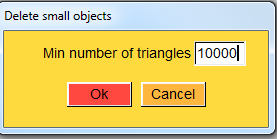
\includegraphics[scale=0.5]{images/Edit_selected_objects/Delete_small_1.png}
 \captionof{figure}{Delete small objects window}
 \end{minipage} 
\noindent




\subsection{Threshold : a given volume}
\noindent
\begin{minipage}{0.5\textwidth}
Using this option, you may delete selected objects smaller than a given volume.

\end{minipage}    
\begin{minipage}{0.5\textwidth}\centering
  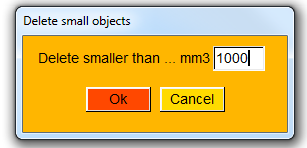
\includegraphics[scale=0.5]{images/Edit_selected_objects/Delete_small_2.png}
 \captionof{figure}{Delete small objects window 2}
 \end{minipage} 
\noindent

